\chapter{Implementarea sistemului IORA}\label{chap:implementare}
\indent\par
Sistemul propus în lucrarea de față, denumit IORA, a fost construit pornind de la o arhitectură modulară formată din trei componente cheie: modulul de preluare a datelor (\textit{Input Module}), fluxul de procesare (\textit{Processing Pipeline}) și modulul de logică a aplicației (\textit{Application Logic Module}). Pentru a oferi flexibilitate și a respecta principiile de proiectare extensibilă specifice conceptului de \textit{clean code}~\cite{codecomplete}, modulul de intrare și cel de logică a aplicației utilizează polimorfismul prin expunerea unor interfețe abstracte.

Această abordare decuplată permite diferitelor aplicații să integreze nucleul sistemului într-un mod elegant, implementând comportamente personalizate și adaptate la mediul de execuție, fără a modifica codul de bază. De exemplu, modulul de intrare poate fi extins pentru a prelua fluxuri video de la o cameră atașată mediului de execuție, fie prin intermediul \textit{socket-urilor}. În mod similar, modulul de logică a aplicației poate fi personalizat pentru a declanșa acțiuni specifice precum trimiterea unor notificări automate prin \textit{e-mail}, sau acționarea unor echipamente \textit{hardware}, în cazul unui sistem integrat.

În contrast, fluxul de procesare este încapsulat ca o unitate de execuție independentă și de sine stătătoare, neexpunând nicio interfață publică destinată extinderii structurale.

În continuare, acest capitol descrie arhitectura și tehnologiile utilizate în implementarea aplicației prezentate alături de o descriere tehnică a fiecărui modul.

\section{Arhitectura sistemului}
\indent\par
Sistemul IORA este organizat pe trei niveluri logice care corespund celor trei module introduse la începutul capitolului: nivelul de achiziție a datelor, nivelul de procesare și nivelul de logică a aplicației. Această stratificare urmărește o separare clară a responsabilităților, fiecare nivel comunicând cu cel adiacent exclusiv prin structuri de date simple, independente de bibliotecile externe folosite în implementare. Decuplarea astfel obținută permite ca un nivel să fie înlocuit sau extins fără a afecta restul sistemului.

\subsection{Diagrama de componente}
\indent\par
Diagrama de componente, prezentată în Figura~\ref{fig:componente}, surprinde cele trei module și fluxul de date dintre ele. Modulul de intrare expune interfața \texttt{ICaptureManager} și produce, indiferent de sursa fizică a datelor, obiecte de tip \texttt{Frame}. Aceste obiecte constituie singurul punct de contact dintre modulul de intrare și fluxul de procesare, eliminând orice dependență a nucleului de natura sursei de captură.

Fluxul de procesare consumă obiectul \texttt{Frame} și aplică, în mod secvențial, cele trei etape ale procesului de recunoaștere: localizarea plăcuței, segmentarea caracterelor și recunoașterea acestora. Rezultatul produs (șirul de caractere recunoscut, însoțit de metadatele asociate) este transmis mai departe către modulul de logică a aplicației, care decide acțiunea declanșată în funcție de contextul de execuție.

\begin{figure}[H]
  \centering
  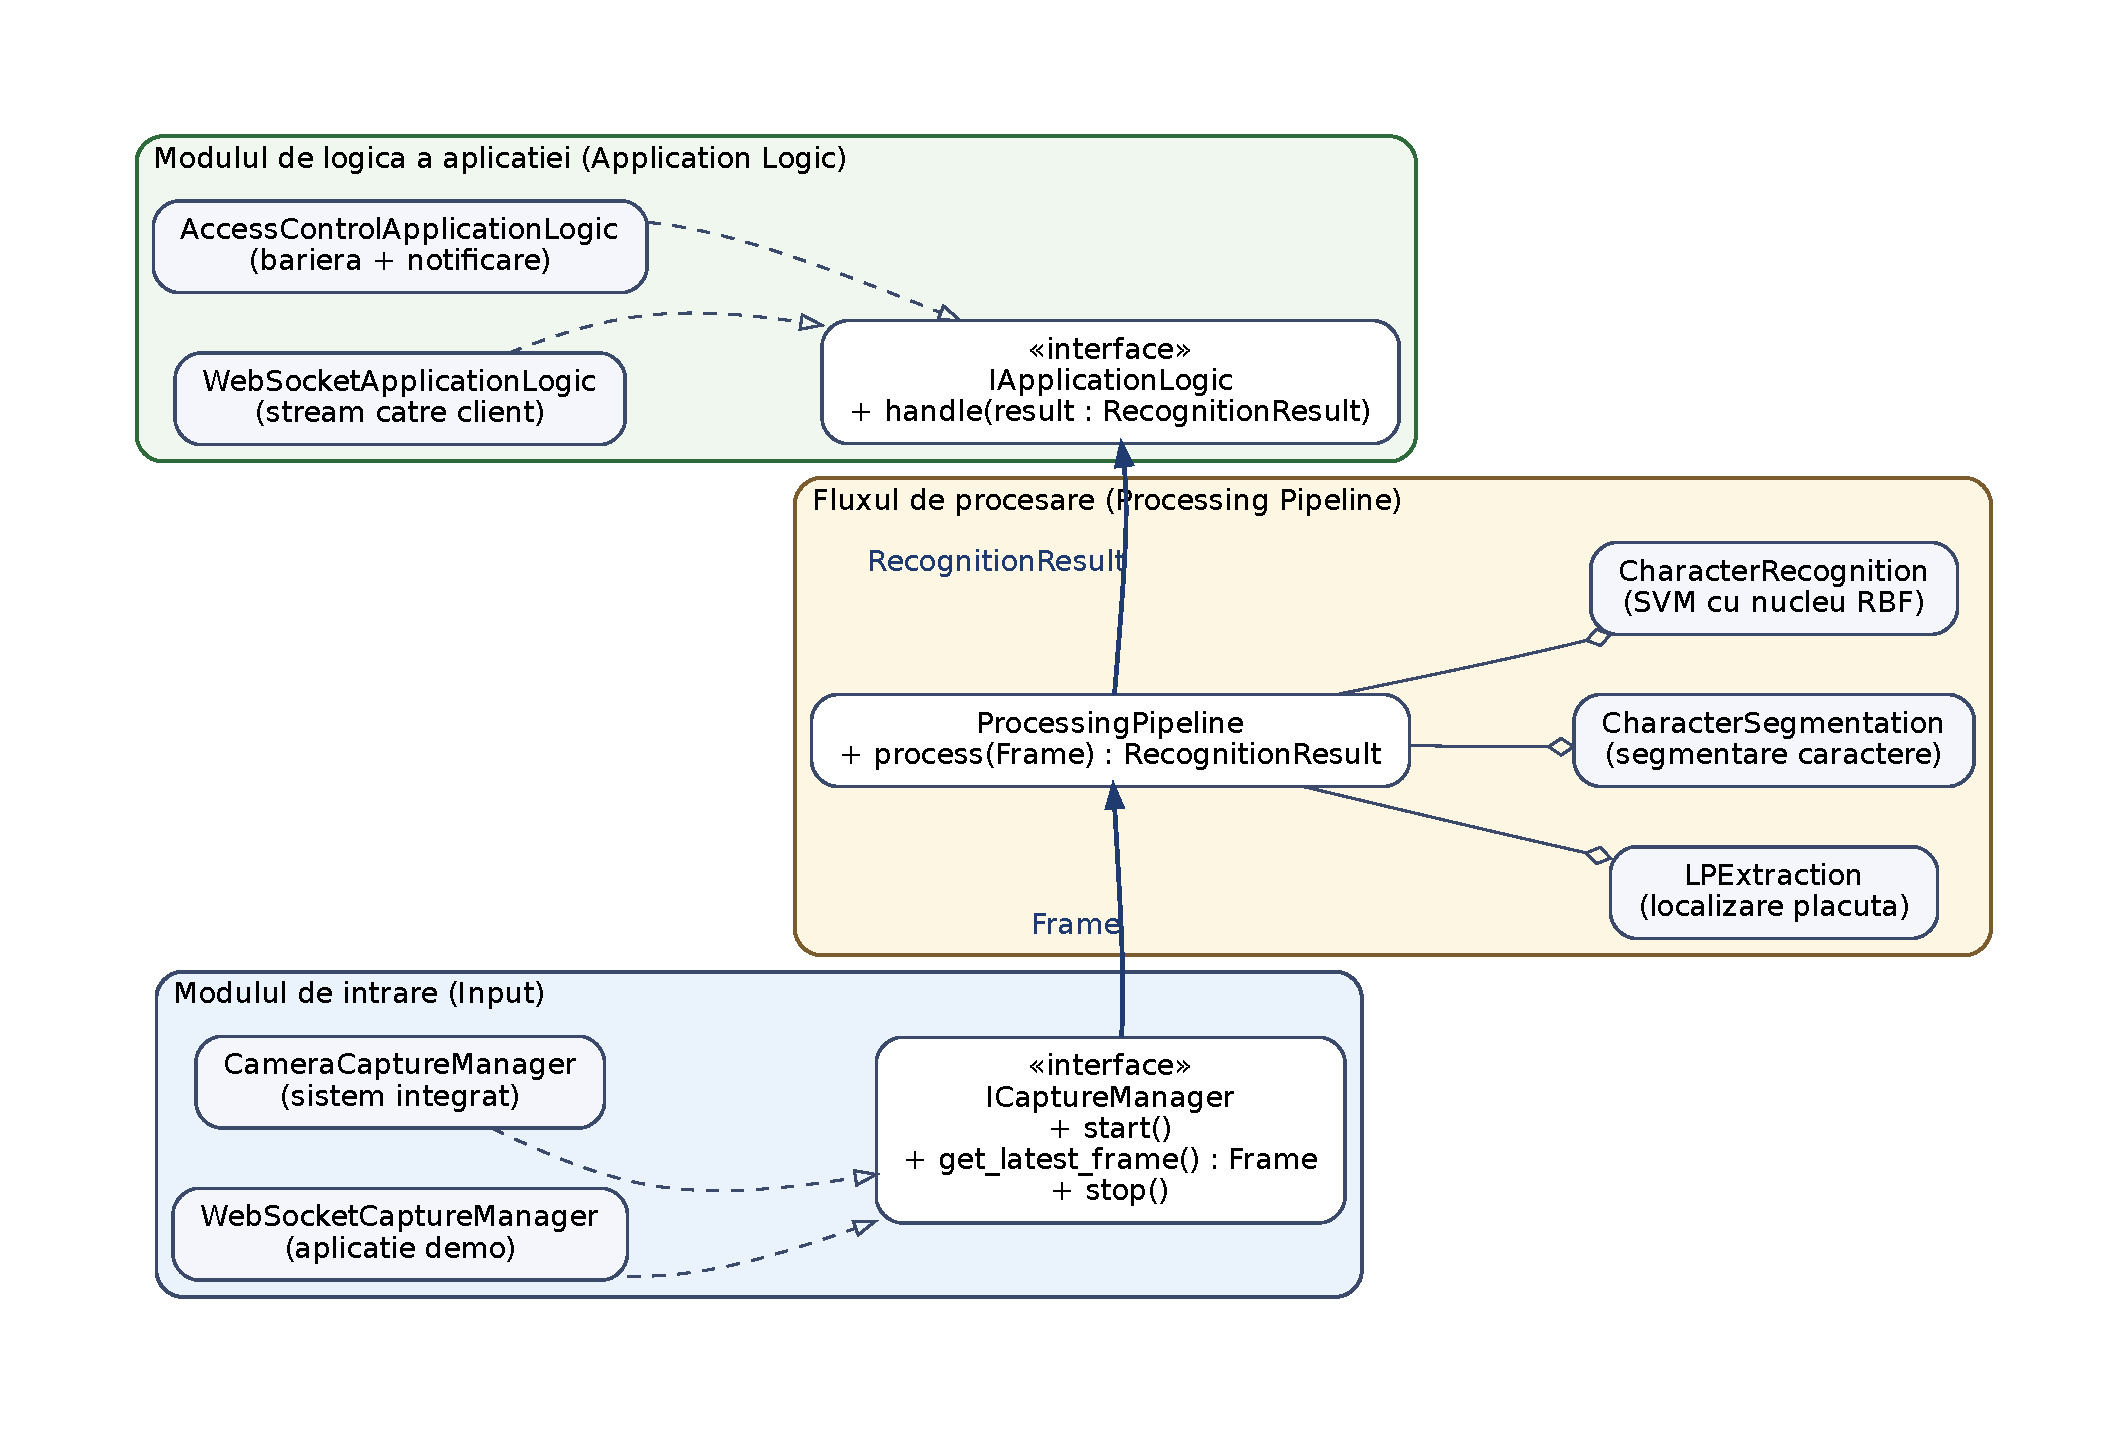
\includegraphics[width=0.9\linewidth]{figures/iora_componente.pdf}
  \caption{Diagrama de componente a sistemului IORA: modulele de intrare,
    procesare și logică a aplicației, împreună cu structurile de date
    \texttt{Frame} și \texttt{RecognitionResult} care le decuplează.}
  \label{fig:componente}
\end{figure}

\subsection{Actori și cazuri de utilizare}
\indent\par
În cadrul scenariului de utilizare vizat, sistemul interacționează cu mai mulți actori, atât umani, cât și automați. Actorul uman principal este operatorul, responsabil de configurarea și monitorizarea sistemului. Actorii automați sunt reprezentați de echipamentele și serviciile care consumă rezultatul recunoașterii: sistemul de barieră (acționat în urma unei recunoașteri valide) și serviciul de notificare (care transmite alerte, de exemplu prin \textit{e-mail}).

Principalele cazuri de utilizare sunt: monitorizarea fluxului video de la sursa de captură, citirea automată a numărului de înmatriculare dintr-un cadru și declanșarea unei acțiuni asociate (ridicarea barierei sau emiterea unei notificări) pe baza rezultatului recunoașterii. Pentru aplicația demonstrativă, se adaugă cazul de utilizare al transmiterii rezultatelor către un client extern prin intermediul unei conexiuni \textit{WebSocket}. Aceste cazuri de utilizare, împreună cu actorii implicați, sunt sintetizate în Figura~\ref{fig:usecase}.

\begin{figure}[H]
  \centering
  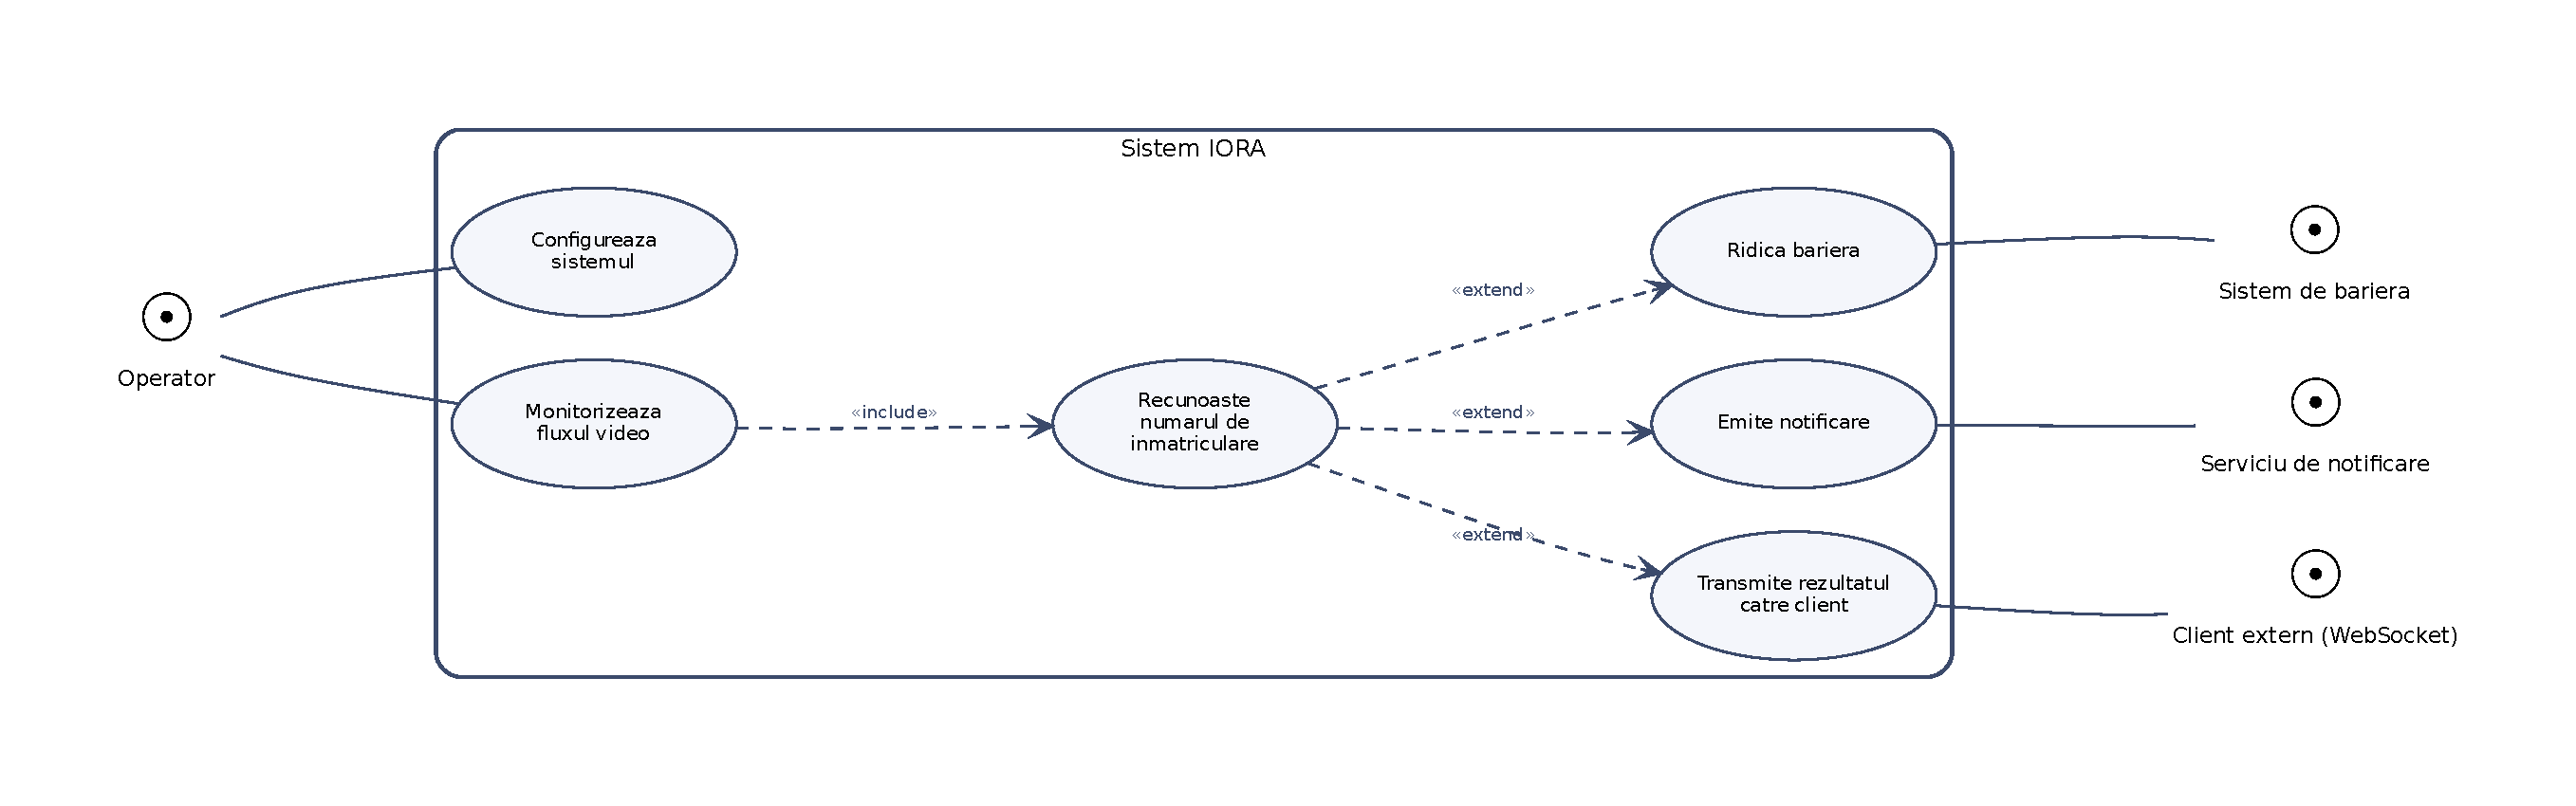
\includegraphics[width=\linewidth]{figures/iora_usecase.pdf}
  \caption{Diagrama cazurilor de utilizare a sistemului IORA, cu operatorul
    drept actor uman principal și sistemele consumatoare ale rezultatului
    recunoașterii drept actori automați.}
  \label{fig:usecase}
\end{figure}

\subsection{Diagrama de clase}
\indent\par
Diagrama de clase din figura~\ref{fig:clase} reflectă, la nivel structural, aceeași stratificare introdusă de diagrama de componente: interfețele \texttt{ICapture\-Manager} și \texttt{IApplication\-Logic} delimitează marginile extensibile ale sistemului, fiecare având două realizări concrete (una pentru sistemul integrat, una pentru aplicația demonstrativă), în timp ce nucleul de procesare este modelat prin clasa \texttt{ProcessingPipeline}, care agregă cele trei etape ale recunoașterii (\texttt{LPExtraction},\- \texttt{CharacterSegmentation},\- \texttt{CharacterRecognition}). Tipurile de date proprii \texttt{Frame} și \texttt{RecognitionResult} apar ca dependențe la marginile fluxului, marcând explicit decuplarea nucleului de detaliile de implementare ale surselor de captură și ale acțiunilor declanșate de aplicație.

\begin{figure}[H]
  \centering
  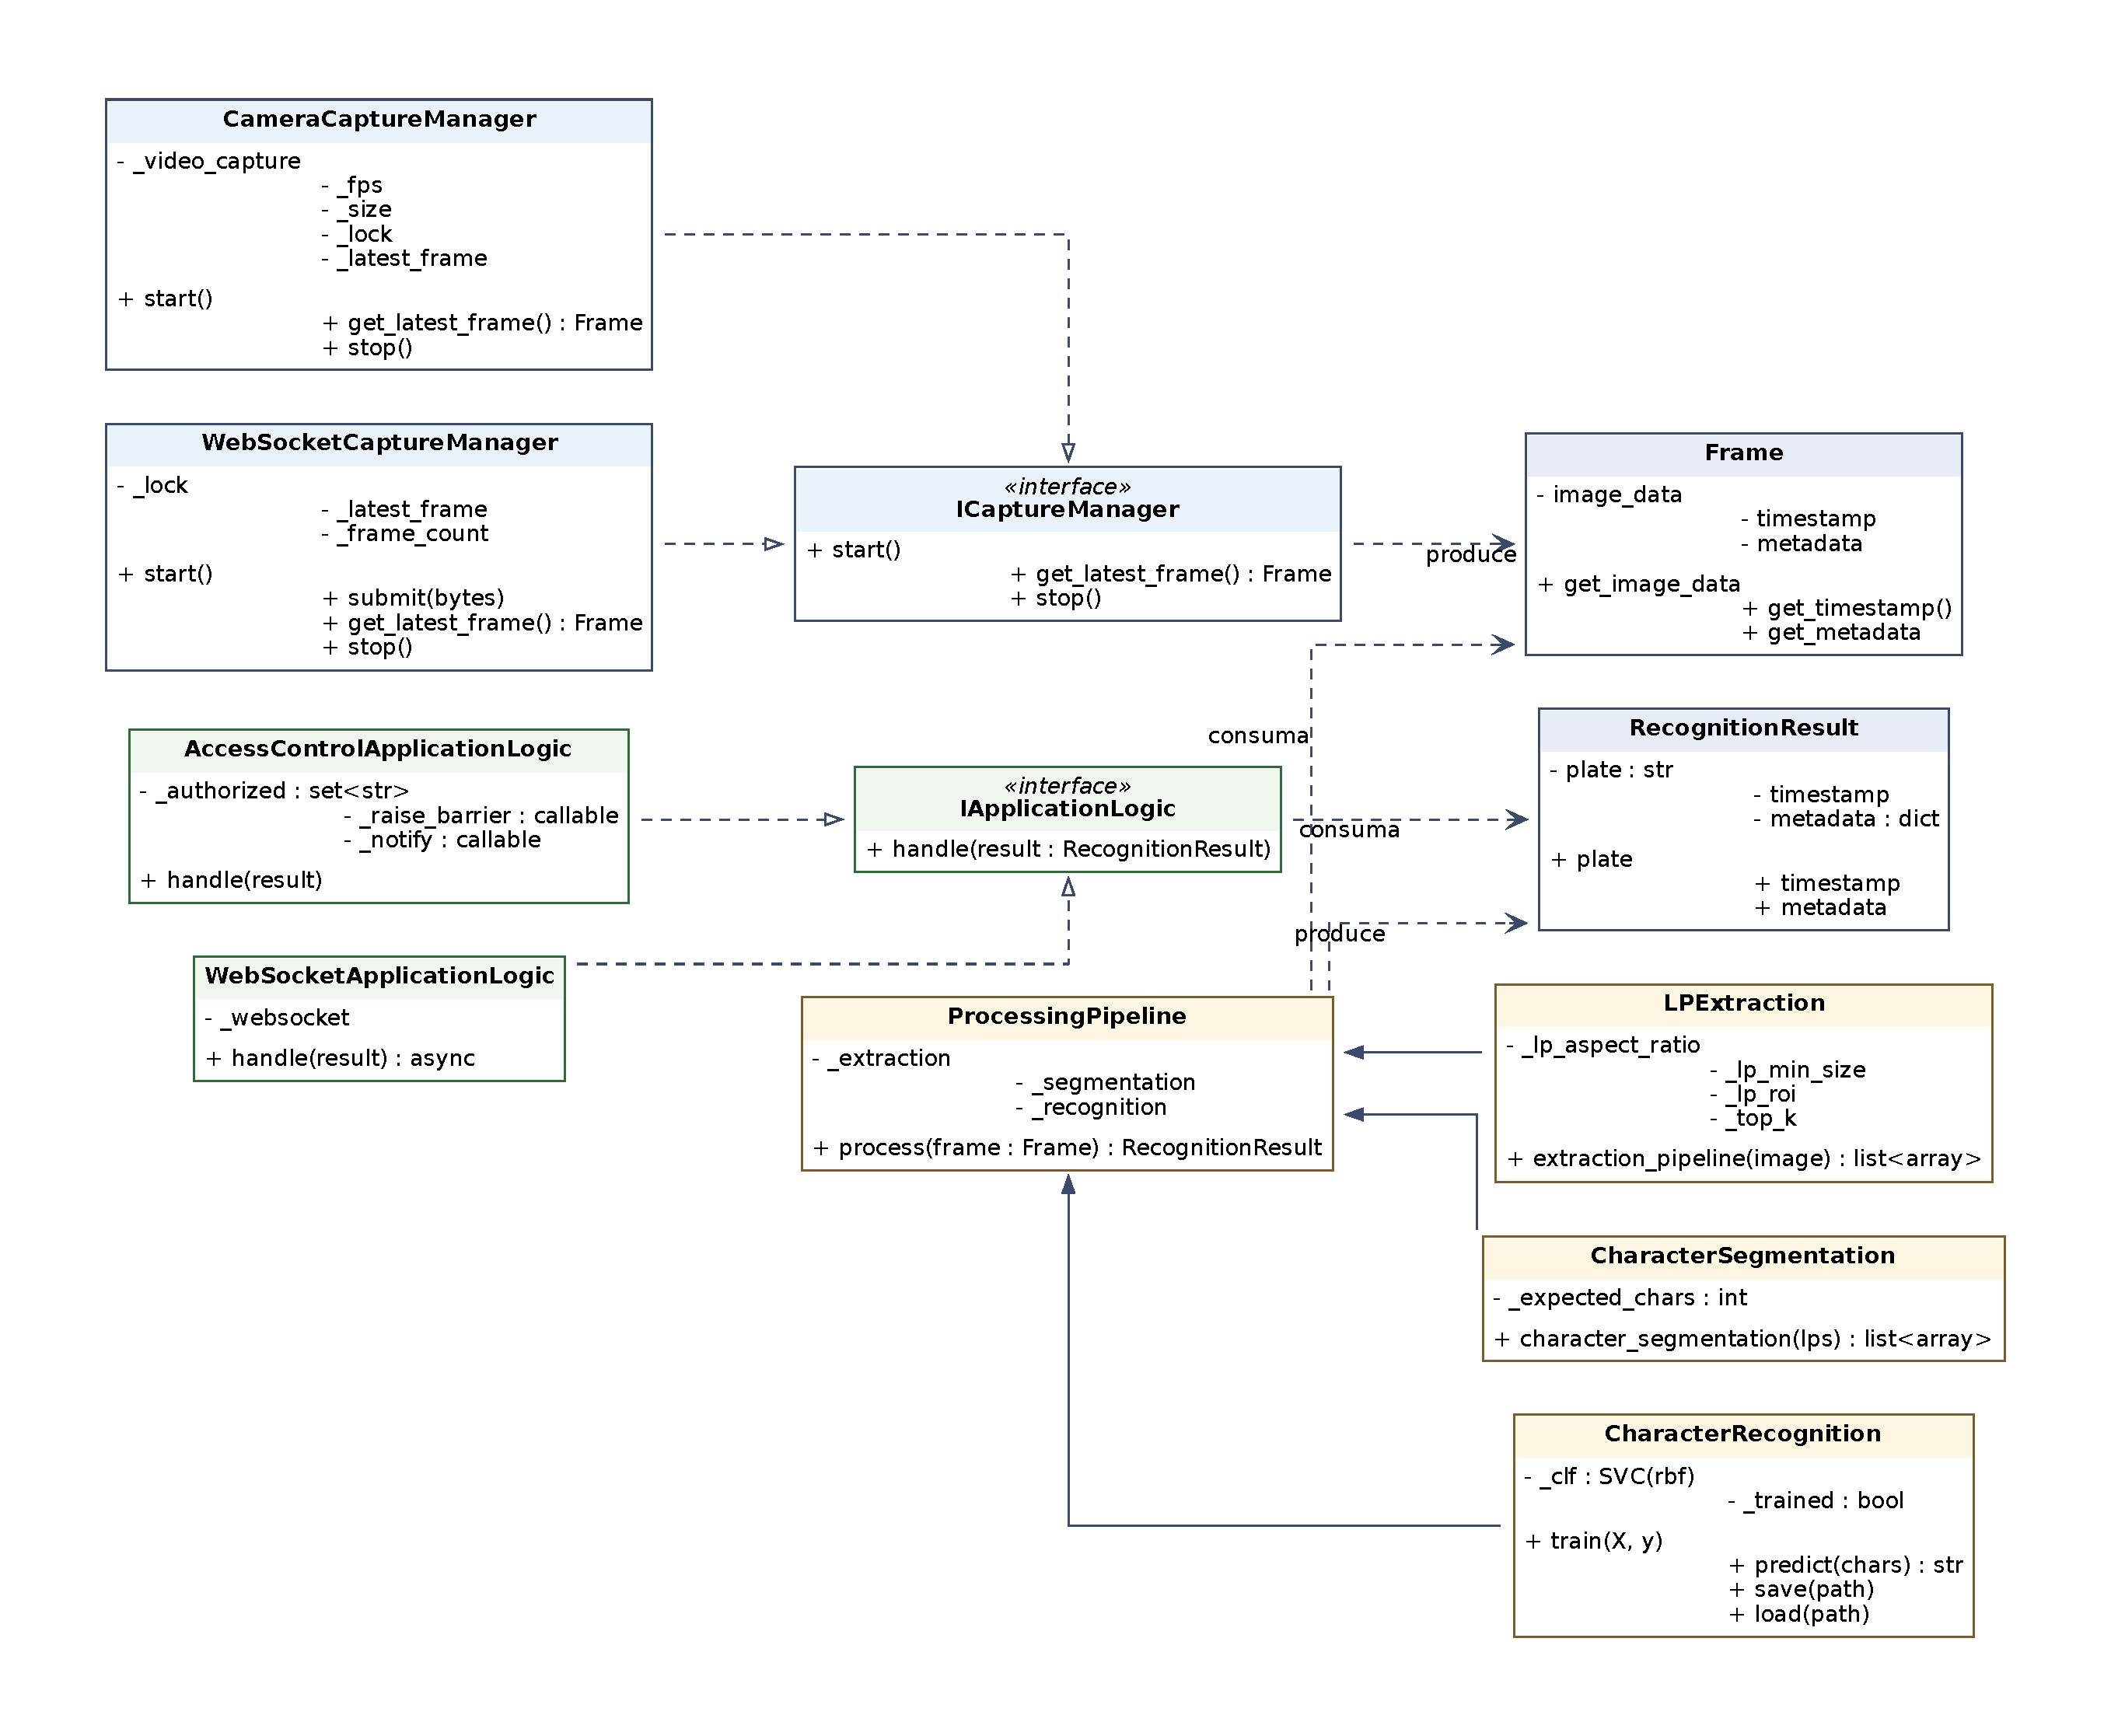
\includegraphics[width=\linewidth]{figures/iora_clase.pdf}
  \caption{Diagrama de clase a sistemului IORA: interfețele extensibile, realizările lor concrete și agregarea celor trei etape de procesare în \texttt{ProcessingPipeline}.}
  \label{fig:clase}
\end{figure}

\subsection{Decizii de proiectare}
\indent\par
Proiectarea bazată pe principiile arhitecturale menționate anterior sugerează natura componentelor: modulele de la margini interacționează direct cu mediul de execuție și sunt, prin urmare, cele mai susceptibile la variații, motiv pentru care comportamentul lor este abstractizat prin interfețe conform principiilor de \textit{clean code}~\cite{codecomplete}. În schimb, fluxul de procesare implementează un algoritm stabil, independent de context, care nu beneficiază de pe urma extensibilității.

O a doua decizie de proiectare vizează minimizarea dependențelor la nivelul nucleului și definirea unor tipuri de date proprii. Această alegere consolidează portabilitatea sistemului și permite adoptarea sa în contexte de rulare diferite, de la sisteme integrate cu resurse limitate până la servere care deservesc o aplicație web.

\section{Tehnologii}
\indent\par
Alegerea limbajului a fost făcută pe considerente practice, așadar întreg sistemul a fos implementat în Python 3.14.4 în detrimenul unui limbaj compilat precum C++. Această decizie a fost motivată de gradul ridicat de adopție a ecosistemului Python în cadrul sistemelelor integrate, precum și de flexibilitatea și viteza de dezvoltare specifice oferite de un limbaj dinamic. De asemenea, librăriile necesare implementării modului de procesare se bazează pe nuclee scrise în C.

Pentru a oferi o structură clară, tehnologiile utilizate au fost împărțite în două categorii: cele fundamentale, necesare dezvoltării nucleului și cele adiționale, specifice dezvolării aplicației finale.

\subsection{Nucleu}
\indent\par
Din punct de vedere tehnologic, implementarea nucleului se bazează pe un ecosistem minimalist de dependențe. Tehnologiile de bază utilizate sunt:
\begin{itemize}
  \item{OpenCV 4.13.0}
  \item{numpy 2.4.2}
  \item{scikit-learn 1.8.0}
  \item{matplotlib-base 3.10.9}
\end{itemize}

\subsection{Nivelul de aplicație}
\indent\par
După cum am menționat, dependențele necesare dezvoltării aplicației finale sunt opționale, acestea depinzând strict de contextul aplicației dorite. Pentru aplicația propusă, dependențele sunt:
\begin{itemize}
  \item{fastapi 0.135.4}
  \item{websockets 15.0.1}
\end{itemize}

\section{Detalii tehnice}
\indent\par
În cele ce urmează va fi prezentată o descriere detaliată a arhitecturii fiecărui modul, abordând aspecte precum interfețele de programare expuse, deciziile de proiectare și implementarea propriu-zisă.

Pentru modulele extensibile, se va realiza o paralelă între implementarea în cadrul unui sistem integrat și implementarea concretă realizată în cadrul aplicației demonstrate.

\subsection{Modulul de intrare}
\indent\par
Achiziția datelor de intrare reprezintă punctul de plecare al sistemului. Acest modul are rolul exclusiv de a prelua informația brută și de a o expune către fluxul de procesare. În continuare vor fi prezentate elementele atât abstracte cât și concrete ale acestei componente.

\subsubsection{Interfața ICaptureManager}
\indent\par
Interfața \texttt{ICaptureManager} este definită prin trei metode esențiale. Primele două, \texttt{start} și \texttt{stop}, gestionează ciclul de viață al sistemului de captură, ocupându-se de inițializarea și, respectiv, de eliberarea resurselor asociate acestuia. Cea de-a treia metodă, \texttt{get\_latest\_frame}, returnează cel mai recent cadru preluat, încapsulat într-un obiect de tip \texttt{Frame}.
\begin{verbatim}
    def start(self) -> None:
        pass

    def get_latest_frame(self) -> Frame:
        pass

    def stop(self) -> None:
        pass
\end{verbatim}

\subsubsection{Sistem integrat}
\indent\par
Pentru scenariul rulării pe un sistem integrat, a fost realizată o implementare exemplificativă, clasa \texttt{CameraCaptureManager}, responsabilă de preluarea cadrelor de la o cameră conectată direct la dispozitiv.

Implementarea se bazează pe biblioteca OpenCV pentru a media interacțiunea cu subsistemul de captură video al sistemului de operare. Identificarea sursei fizice se realizează prin intermediul indexului de dispozitiv asociat camerei, transmis ca parametru constructorului clasei.

Pe lângă indexul de dispozitiv, clasa expune următoarele atribute private:
\begin{itemize}
  \item{\texttt{\_video\_capture} - obiectul OpenCV prin care se realizează comunicarea cu camera;}
  \item{\texttt{\_fps} - numărul de cadre pe secundă raportat de dispozitiv;}
  \item{\texttt{\_size} - rezoluția cadrelor preluate, dedusă din primele cadre citite;}
  \item{\texttt{\_lock} - obiect necesar pentru sincronizarea accesului la cel mai recent cadru.}
\end{itemize}

Metoda \texttt{get\_latest\_frame} a fost proiectat astfel încât să returneze întotdeauna cel mai recent cadru disponibil. Această cerință este esențială într-un context de procesare în timp real: întrucât bibliotecile de captură mențin o memorie internă, citirea secvențială a cadrelor ar introduce o latență cumulativă, returnând cadre deja învechite. Pentru a evita acest fenomen, un fir de execuție (\textit{thread}) dedicat preia continuu cadrele de la cameră, păstrând disponibil doar cel mai recent dintre acestea. Accesul concurent la resursa partajată este sincronizat printr-un mecanism de tip \textit{lock}.

\subsubsection{Aplicație demonstrativă}
\indent\par
În cadrul aplicației demonstrative, sursa de captură nu este o cameră atașată direct dispozitivului, ci un flux video transmis în timp real (\textit{live-feed}) printr-o conexiune \textit{WebSocket}. Această implementare menține o conexiune persistentă prin care cadrele sosesc continuu de la un client extern, le decodează și le încapsulează în același obiect \texttt{Frame}. La fel ca în cazul implementării pentru sistemul integrat, doar cel mai recent cadru recepționat este păstrat disponibil, evitând acumularea unei latențe în contextul procesării în timp real.

\subsection{Fluxul de procesare}
\indent\par

\subsubsection{Considerații preliminare}
\indent\par
Precum am menționat când am definit contextul aplicației, există o diversitate ridicată în privința formatului, a paletei cromatice de fond, a dimensiunilor relative și a fontului caracterelor. Tocmai din aceste motive, în prezenta lucrare a fost exclusă de la bun început orice abordare bazată pe segmentarea culorii, deși aceasta este frecvent utilizată în literatura de specialitate. Generalizarea acestor abordări către scenariul nostru ar fi necesitat menținerea unui catalog de palete pentru fiecare format admis, ceea ce ar fi introdus o sursă suplimentară de erori și ar fi diminuat capacitatea de adaptare a sistemului.

\subsubsection{Localizarea plăcuței de înmatriculare}
\indent\par
În capitolul teoretic dedicat acestui sub-sistem au fost menționate trei abordări: bazate pe culoare, pe contururi sau pe textură. După cum am menționat anterior, cele bazate pe culoare nu sunt o variantă fiabilă deoarece pe teritorul României există patru combinații cromatice posibile care definesc un număr de înmatriculare valid.

Pe de altă parte, metodele bazate pe textură prezintă un grad al robusteții mai scăzut față de cele bazate pe contururi. Deși ambele categorii pornesc de la aceeași observație, anume că zona caracterelor produce o concentrare de tranziții de intensitate, ele diferă fundamental prin criteriul de decizie folosit pentru a confirma o regiune drept plăcuță.

Abordările texturale se folosesc de prezența caracterelor drept caracteristică principală a numărului de înmatriculare. Acest descriptor nu este unul robust pentru cazul general, deoarece văile care separă două caractere diferă de la format la format. Totodată, sensibilitatea la zgomot reprezintă o limitare majoră a acestor metode. O imagine degradată sau prezența unor umbre poate compromite analiza proiecțiilor verticale, ducând la detectarea eronată a unor văi inexistente.

În contrast, metodele bazate pe contururi tratează concentrarea de tranziții doar ca pe un indiciu, lăsând decizia finală în seama unei constante geometrice: forma dreptunghiulară cu un raport de aspect cunoscut. Deoarece acest criteriu nu depinde de modul în care sunt distribuite caracterele, ci de forma regiunii, el rămâne stabil indiferent de fontul, dimensiunea sau numărul caracterelor.

Pornind de la aceste considerente, etapa de localizare a fost implementată în clasa \texttt{LPExtraction}, parametrizată prin raportul de aspect admis pentru o plăcuță (\texttt{lp\_aspect\_ratio}), aria minimă a unei regiuni candidat (\texttt{lp\_min\_size}), o regiune de interes opțională (\texttt{lp\_roi}) și numărul de candidați returnați (\texttt{top\_k}). Fluxul de procesare urmează etapele clasice ale abordării pe contururi, descrise în capitolul~\ref{chap:localizare}, adaptate contextului autohton.

Preprocesarea începe, dacă este definită, cu decuparea regiunii de interes, urmată de conversia în tonuri de gri și de aplicarea unui filtru median pentru atenuarea zgomotului. Asupra imaginii filtrate se aplică operatorul Sobel pe direcția orizontală, evidențiind muchiile verticale generate de caractere.

Rezultatul este binarizat prin metoda Otsu în variantă inversată conformându-se astfel cu formatul așteptat de funcția de extragere a contururilor. Asupra imaginii binare se aplică o operație morfologică de deschidere, urmată de o dilatare cu un nucleu orizontal a cărui lățime este direct proporțională cu lățimea imaginii. Scopul dilatării este de a unii elementele plăcuței care au fost separate în pașii anteriori.

După toate acestea se extrag contururile externe, iar dreptunghiurile lor de încadrare sunt filtrare pe baza raportului de aspect si a ariei minime, eliminiând regiunile necorespunzătoare.

\begin{verbatim}
    greyscale = cv.cvtColor(array, cv.COLOR_BGR2GRAY)
    median = self._helper.median_filter(array=greyscale)
    sobel = self.sobel(median)
    thresh = self._helper.otsu_thresholding(sobel)
    thresh = cv.bitwise_not(thresh)
    open_image = self._helper.opening(thresh)
    dilated_image = self._helper.dilation(open_image)
    bounding_box = self._helper.find_countours(
        dilated_image,
        self._lp_aspect_ratio,
        self._lp_min_size
    )
\end{verbatim}

Datorită experimentelor a putut fi observat faptul că, în majoritatea cazurilor plăcuțele erau fragmentate în două sau chiar trei bucăți. Așadar a fost necesară implementarea unei metode de reuniune a acestor fragmente pornind de la poziția lor în cadrul imaginii. Fiecare dreptunghi de încadrare extras de pasul anterior este extins în interiorul imaginii cu o margine fixă, iar dacă două dintre dreptunghiurile inițiale se suprapun în urma extinderii ele sunt unite.

În final, candidații rămași sunt ordonați după densitatea de muchii din interiorul lor, iar primii \texttt{top\_k} sunt returnați. Returnarea mai multor candidați, în locul unuia singur, constituie o decizie de proiectare deliberată: ea permite etapei următoare de segmentare să recupereze eventualele erori de localizare, alegând candidatul care conduce la cea mai plauzibilă segmentare.

Rezultatul acestei etape poate fi observat în Figura~\ref{fig:rezultat_localizare} care prezintă cele trei regiuni de interes extrase de modul în momentul în care acesta este construit cu parametrul \texttt{top\_k}$=3$.

\begin{figure}[H]
  \centering
  \begin{subfigure}[c]{0.40\linewidth}
    \centering
    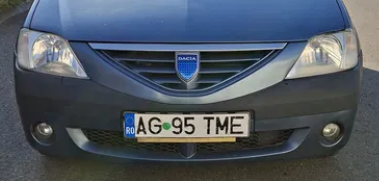
\includegraphics[width=\linewidth]{figures/AG95TME.png}
    \caption{Cadrul de intrare}
  \end{subfigure}
  \hfill
  \begin{subfigure}[c]{0.18\linewidth}
    \centering
    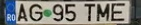
\includegraphics[width=\linewidth]{figures/AG95TME.png_lp_0.jpg}
    \caption{Candidatul 1}
  \end{subfigure}
  \hfill
  \begin{subfigure}[c]{0.18\linewidth}
    \centering
    
\includegraphics[width=\linewidth]{figures/AG95TME.png_lp_1.jpg}
    \caption{Candidatul 2}
  \end{subfigure}
  \hfill
  \begin{subfigure}[c]{0.18\linewidth}
    \centering
    
\includegraphics[width=\linewidth]{figures/AG95TME.png_lp_2.jpg}
    \caption{Candidatul 3}
  \end{subfigure}
  \caption{Imaginea inițială și cele 3 elemente extrase în momentul rulării modulului de localizare cu \texttt{top\_k}$=3$.}
  \label{fig:rezultat_localizare}
\end{figure}

\subsubsection{Segmentarea caracterelor}
\indent\par
Etapa de segmentare primește candidații de plăcuță produși de etapa de localizare și are ca scop izolarea fiecărui caracter într-o imagine distinctă. Dintre tehnicile prezentate în capitolul~\ref{chap:segmentare}, a fost adoptată analiza contururilor, combinată cu utilizarea cunoștințelor apriori privind aspectul caracterelor. Această alegere a fost preferată unei abordări bazate pe analiza proiecțiilor care, deși oferă o reprezentare unidimensională compactă a distribuției pixelilor de prim-plan, depinde de existența unor văi suficient de adânci între caracterele adiacente. Pe plăcuțele reale, înclinarea de câteva grade și spațierea neuniformă a caracterelor fac ca aceste văi să se estompeze, fuzionând simboluri vecine într-un singur segment. Decizia la nivelul fiecărei componente conexe în parte rămâne, în schimb, independentă de unghiul de înclinare și de spațierea dintre simboluri, comportament confirmat de comparația cantitativă prezentată în secțiunea de experimente.

Pipeline-ul de segmentare începe cu restrângerea decupajului la corpul efectiv al plăcuței, eliminând contextul reținut eronat în etapa de localizare, precum fragmentele de caroserie sau cadrul plăcuței. Restrângerea se realizează fie prin selectarea celei mai mari componente conexe luminoase, corespunzătoare fundalului uniform al plăcuței, fie, atunci când aceasta nu este concludentă, prin detectarea benzii de caractere: elementele de înălțime plauzibilă sunt grupate după coordonata lor verticală, iar decupajul este redus la dreptunghiul de încadrare al grupului dominant.

Corpul astfel obținut este binarizat printr-un prag adaptiv gaussian în variantă inversată (\texttt{adaptiveThreshold}), care compensează variațiile locale de iluminare de-a lungul plăcuței, obținând caracterele drept prim-plan alb. Din imaginea binară se extrag contururile externe, iar dreptunghiurile lor de încadrare constituie casetele-candidat pentru caractere. Atunci când numărul de contururi este insuficient (sub trei), imaginea este erodată ușor, iar extragerea este reluată, separând caracterele unite accidental prin zgomot.

Casetele-candidat sunt apoi filtrate printr-o succesiune de criterii derivate din aspectul așteptat al unui caracter. Un prag de contrast intern, calculat ca abaterea standard a intensităților din interiorul casetei raportată la un prag Otsu determinat pe ansamblul casetelor, elimină regiunile uniforme precum reziduurile cadrului. Constrângerile de înălțime relativă (între $0{,}40$ și $0{,}95$ din înălțimea plăcuței) și de raport de aspect ($w/h$ între $0{,}08$ și $1{,}3$) elimină structurile prea mici sau cu geometrie implauzibilă, pragul inferior fiind suficient de permisiv pentru a păstra caractere înguste precum cifra \texttt{1}. În final, casetele care ating marginile laterale ale decupajului sunt respinse, anulând fragmentele de cadru tăiate, iar o trecere de consistență păstrează doar casetele a căror înălțime se află în jurul valorii mediane (între $0{,}55$ și $1{,}45$ din aceasta).

\begin{verbatim}
    thresholded = cv.adaptiveThreshold(
        greyscale, 255, cv.ADAPTIVE_THRESH_GAUSSIAN_C,
        cv.THRESH_BINARY_INV, block, 2)
    contours = self._helper.find_countours(
        thresholded, aspect_ratio_bounds=(0.04, 2.0))
    for c, s in zip(contours, stds):
        x, y, w, h = c
        if s < std_thr:
            continue
        if not (min_height <= h <= max_height):
            continue
        if not (min_w_h <= w / h <= max_w_h):
            continue
        if x < border_margin or (x + w) > (W - border_margin):
            continue
        kept.append((x, y, w, h))
\end{verbatim}

Caracterele lipite, care produc o singură casetă vizibil mai lată decât înaltă ($w > 1{,}2\,h$), sunt separate ulterior prin metoda \texttt{\_split\_wide\_blobs}: în interiorul casetei se calculează proiecția verticală pe coloane, iar tăierea se face în dreptul minimelor locale (văile dintre caractere), numărul de tăieturi fiind estimat din raportul de aspect al casetei. Spre deosebire de o abordare globală bazată pe proiecții, profilul este aici folosit strict local, pentru a împărți o regiune deja izolată, evitând astfel sensibilitatea profilului global la înclinarea plăcuței.

Deoarece etapa de localizare poate furniza mai mulți candidați de plăcuță, segmentarea este rulată pe fiecare dintre aceștia, iar setul de caractere reținut este cel care obține scorul maxim conform unei funcții de evaluare (\texttt{\_score}). Acest cuplaj prin parametrul \texttt{top\_k} transformă etapa de segmentare într-un mecanism de recuperare a erorilor de localizare: un candidat incorect (de exemplu o regiune de grilaj reținută eronat) va produce o segmentare cu un scor scăzut și va fi astfel respins în favoarea candidatului corect.

Funcția de evaluare valorifică o cunoștință apriori esențială: o plăcuță validă conține un număr cunoscut de caractere, de dimensiuni comparabile și dispuse pe aceeași linie de bază. Scorul integrează, în consecință, trei componente: abaterea numărului de casete detectate față de numărul așteptat (în jur de șapte simboluri pentru formatul autohton), consistența înălțimilor casetelor (caracterele unei plăcuțe au înălțimi similare) și alinierea lor verticală (caracterele împărtășesc aceeași linie de bază). O segmentare care satisface aceste constrângeri primește un scor ridicat, întrucât corespunde tiparului geometric al unei plăcuțe reale.

Rezultatul acestei etape este ilustrat în Figura~\ref{fig:rezultat_segmentare}: pornind de la plăcuța localizată în etapa anterioară, modulul izolează fiecare caracter într-o imagine distinctă, producând cele șapte simboluri care urmează a fi transmise individual etapei de recunoaștere.

\begin{figure}[H]
  \centering
  % TODO: înlocuiește numele fișierelor cu pozele finale
  \begin{subfigure}[b]{0.5\linewidth}
    \centering
    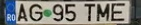
\includegraphics[width=\linewidth]{figures/AG95TME.png_lp_0.jpg}
    \caption{Plăcuța localizată}
  \end{subfigure}

  \vspace{0.8em}

  \begin{subfigure}[b]{0.12\linewidth}
    \centering
    
\includegraphics[width=\linewidth]{figures/char_0.jpg}
  \end{subfigure}
  \hfill
  \begin{subfigure}[b]{0.12\linewidth}
    \centering
    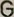
\includegraphics[width=\linewidth]{figures/char_1.jpg}
  \end{subfigure}
  \hfill
  \begin{subfigure}[b]{0.12\linewidth}
    \centering
    
\includegraphics[width=\linewidth]{figures/char_2.jpg}
  \end{subfigure}
  \hfill
  \begin{subfigure}[b]{0.12\linewidth}
    \centering
    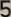
\includegraphics[width=\linewidth]{figures/char_3.jpg}
  \end{subfigure}
  \hfill
  \begin{subfigure}[b]{0.12\linewidth}
    \centering
    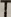
\includegraphics[width=\linewidth]{figures/char_4.jpg}
  \end{subfigure}
  \hfill
  \begin{subfigure}[b]{0.12\linewidth}
    \centering
    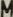
\includegraphics[width=\linewidth]{figures/char_5.jpg}
  \end{subfigure}
  \hfill
  \begin{subfigure}[b]{0.12\linewidth}
    \centering
    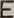
\includegraphics[width=\linewidth]{figures/char_6.jpg}
  \end{subfigure}

  \caption{Rezultatul etapei de segmentare: plăcuța localizată (sus) și cele șapte caractere izolate (jos), fiecare extras într-o imagine distinctă.}
  \label{fig:rezultat_segmentare}
\end{figure}

\subsubsection{Recunoașterea caracterelor}
\indent\par
Ultima etapă a fluxului de procesare atribuie fiecărui caracter segmentat o etichetă, dintr-un alfabet de cifre și litere. Pentru această sarcină a fost ales un clasificator de tip SVM, ale cărui fundamente teoretice au fost prezentate în capitolul~\ref{chap:recunoastere}.

Fiecare caracter este adus la o reprezentare uniformă, independentă de dimensiunea sa originală. Imaginea este mai întâi adusă la o formă pătrată prin completarea laturii mai scurte cu o bordură, apoi redimensionată la o rezoluție fixă de $28 \times 28$ pixeli. Asupra acestei imagini se calculează un descriptor de tip HOG, pe o fereastră de $28 \times 28$ cu celule de $7 \times 7$ pixeli, blocuri de $14 \times 14$ cu pas de $7$ pixeli și $9$ intervale de orientare, rezultă un vector de $324$ de trăsături. Această reprezentare, care surprinde distribuția locală a orientărilor muchiilor în loc de intensitatea brută a pixelilor, constituie intrarea clasificatorului.

Predicția nu se reduce la atribuirea independentă a etichetei celei mai probabile fiecărui caracter, ci valorifică o cunoștință apriori privind formatul plăcuțelor. Atunci când numărul de caractere segmentate corespunde unui format cunoscut, decodarea se realizează poziție cu poziție, restrângând la fiecare poziție mulțimea etichetelor admise (cifră sau literă) și alegând eticheta cu marginea maximă raportată de funcția de decizie a clasificatorului. Pentru lungimile ambigue, în care același număr de caractere admite mai multe tipare, fiecare tipar este evaluat separat, iar varianta cu marginea medie cea mai mare este reținută. Suplimentar, atunci când segmentarea produce un caracter în plus față de un format așteptat, se încearcă și sub-secvențele obținute prin eliminarea pe rând a câte unui caracter, comparate tot pe baza marginii medii per poziție; astfel, un fragment supra-segmentat, care primește o margine apropiată de zero, este eliminat în favoarea tiparului care se potrivește curat. Dacă numărul de caractere nu corespunde niciunui format cunoscut, se revine la atribuirea neconstrânsă a etichetei celei mai probabile.

\subsection{Nivelul de aplicație}
\indent\par
Modulul de logică a aplicației constituie, alături de modulul de intrare, una dintre marginile extensibile ale sistemului. Rolul său este de a consuma rezultatul produs de fluxul de procesare și de a declanșa acțiunea corespunzătoare contextului de execuție.

\subsubsection{Sistem integrat}
\indent\par
În scenariul unui sistem integrat, modulul de logică a aplicației acționează direct asupra mediului fizic. O implementare reprezentativă este cea a unui punct de control al accesului, în care recunoașterea unui număr de înmatriculare aflat într-o listă de autorizare declanșează ridicarea unei bariere auto prin acționarea echipamentului \textit{hardware} corespunzător. Aceeași implementare poate emite, în paralel, notificări automate, de exemplu prin \textit{e-mail}, către un operator sau către un sistem de evidență, atât pentru accesele autorizate, cât și pentru tentativele neautorizate. Caracterul abstract al interfeței permite combinarea liberă a unor astfel de acțiuni, fără modificarea nucleului.

\subsubsection{Aplicație demo}
\indent\par
% DE SCHIMBAT
Pentru aplicația demonstrativă, modulul de logică a aplicației nu acționează asupra unui echipament fizic, ci expune rezultatele recunoașterii către un client extern. Implementarea se bazează pe biblioteca \textit{FastAPI}, care oferă infrastructura unui server web, și pe protocolul \textit{WebSocket}, ales pentru capacitatea sa de a menține o conexiune bidirecțională persistentă. Prin intermediul acestei conexiuni, rezultatele procesării sunt transmise în timp real către interfața clientului, pe măsură ce sunt produse de fluxul de procesare, fără a necesita interogări repetate din partea acestuia.
